% answers.tex —— 1977 年·北京卷·文科 · 参考答案与详细解析片段
% 由 tools/generate_projects.py 依来源总账自 1977/1977_数学真题_北京文_试题.md + 1977/1977_数学真题_北京文_解析正文.md + 1977/1977_数学真题_北京文_答案要点.md 生成，勿手改（改源 MD 后重跑）


\begin{gktip}
固定源为 A3 单页题面，未附答案页；下列推导由编者独立完成，非官方标准答案。
\end{gktip}

\begin{answer}
\gksolhead{1}{}

\textbf{题目}：

\Needspace{5\baselineskip}
计算：

\nopagebreak[4]
\[
3^0+3^{-1}-\left(1\frac79\right)^{\frac12}.
\]

\Needspace{4\baselineskip}
\textbf{解析}

\nopagebreak[4]
\[
3^0+3^{-1}-\left(1\frac79\right)^{\frac12}
=1+\frac13-\sqrt{\frac{16}{9}}=\frac43-\frac43=0.
\]

\gkanswer{答案：$0$。}

\end{answer}
\begin{answer}
\gksolhead{2}{}

\textbf{题目}：

\Needspace{5\baselineskip}
化简：

\nopagebreak[4]
\[
\frac{\sqrt6+\sqrt2}{\sqrt6-\sqrt2}.
\]

\Needspace{4\baselineskip}
\textbf{解析}

\Needspace{5\baselineskip}
有理化得

\nopagebreak[4]
\[
\frac{\sqrt6+\sqrt2}{\sqrt6-\sqrt2}
=\frac{(\sqrt6+\sqrt2)^2}{6-2}
=\frac{8+4\sqrt3}{4}=2+\sqrt3.
\]

\gkanswer{答案：$2+\sqrt3$。}

\end{answer}
\begin{answer}
\gksolhead{3}{}

\textbf{题目}：

\Needspace{5\baselineskip}
解方程：

\nopagebreak[4]
\[
\frac1{x-1}+1=\frac{4x-2}{x^2-1}.
\]

\Needspace{4\baselineskip}
\textbf{解析}

\Needspace{5\baselineskip}
定义域为 $x\ne\pm1$。同乘 $x^2-1$，得

\nopagebreak[4]
\[
(x+1)+(x^2-1)=4x-2,
\]

\Needspace{5\baselineskip}
即

\nopagebreak[4]
\[
x^2-3x+2=(x-1)(x-2)=0.
\]

舍去 $x=1$，故 $x=2$。

\gkanswer{答案：$x=2$。}

\end{answer}
\begin{answer}
\gksolhead{4}{}

\textbf{题目}：

不查表求 $\sin105^\circ$ 的值。

\Needspace{4\baselineskip}
\textbf{解析}

\nopagebreak[4]
\[
\sin105^\circ=\sin(60^\circ+45^\circ)
=\sin60^\circ\cos45^\circ+\cos60^\circ\sin45^\circ
=\frac{\sqrt6+\sqrt2}{4}.
\]

\gkanswer{答案：$\dfrac{\sqrt6+\sqrt2}{4}$。}

\end{answer}
\begin{answer}
\gksolhead{5}{}

\textbf{题目}：

一个正三棱柱形的零件，它的高是 $10\ \mathrm{cm}$，底面边长是 $2\ \mathrm{cm}$，求它的体积。

\Needspace{4\baselineskip}
\textbf{解析}

\Needspace{5\baselineskip}
正三角形底面积为 $\sqrt3$，所以正三棱柱体积为

\nopagebreak[4]
\[
V=\sqrt3\times10=10\sqrt3\ \mathrm{cm^3}.
\]

\gkanswer{答案：$10\sqrt3\ \mathrm{cm^3}$。}

\end{answer}
\begin{answer}
\gksolhead{6}{}

\textbf{题目}：

一条直线过点 $(1,-3)$，并且与直线 $2x+y-5=0$ 平行，求这条直线的方程。

\Needspace{4\baselineskip}
\textbf{解析}

\Needspace{5\baselineskip}
直线 $2x+y-5=0$ 的斜率为 $-2$。过 $(1,-3)$ 的平行线设为

\nopagebreak[4]
\[
2x+y+c=0.
\]

代入点坐标得 $c=1$，故方程为 $2x+y+1=0$。

\gkanswer{答案：$2x+y+1=0$。}

\end{answer}
\begin{answer}
\gksolhead{7}{}

\textbf{题目}：

证明：等腰三角形两腰上的高相等。

\Needspace{4\baselineskip}
\textbf{解析}

设等腰三角形 $ABC$ 中 $AB=AC$，从 $B\text{、}C$ 分别向对边 $AC\text{、}AB$ 作高，垂足为 $E\text{、}F$。两三角形 $ABE$ 与 $ACF$ 中，$AB=AC$，$\angle BAE=\angle CAF$，且均为直角三角形，故全等。因此对应的高 $BE=CF$，即两腰上的高相等。

\gkanswer{答案：见解析版}

\end{answer}
\begin{answer}
\gksolhead{8}{}

\textbf{题目}：

为了测湖岸边 $A\text{、}B$ 两点的距离，选择一点 $C$，测得 $CA=50$ 米，$CB=30$ 米，$\angle ACB=120^\circ$，求 $AB$。

\Needspace{4\baselineskip}
\textbf{解析}

\Needspace{5\baselineskip}
在 $\triangle ABC$ 中，由余弦定理

\nopagebreak[4]
\[
\begin{aligned}
AB^2&=CA^2+CB^2-2\,CA\cdot CB\cos120^\circ\\
&=50^2+30^2-2\cdot50\cdot30\left(-\frac12\right)=4900.
\end{aligned}
\]

所以 $AB=70$ 米。

\gkanswer{答案：$AB=70$ 米。}

\end{answer}
\begin{answer}
\gksolhead{9}{}

\textbf{题目}：

在 $2$ 和 $30$ 中间插入两个正数，这两个正数插入后使前三个数成等比数列，后三个数成等差数列，求插入的两个数。

\Needspace{4\baselineskip}
\textbf{解析}

\Needspace{5\baselineskip}
设插入的两个正数依次为 $x\text{、}y$。前三个数 $2,x,y$ 成等比数列，所以

\nopagebreak[4]
\[
x^2=2y.
\]

\Needspace{5\baselineskip}
后三个数 $x,y,30$ 成等差数列，所以

\nopagebreak[4]
\[
2y=x+30.
\]

消去 $y$ 得 $x^2=x+30$，即 $(x-6)(x+5)=0$。因 $x>0$，故 $x=6$，再得 $y=18$。

\gkanswer{答案：插入的两个数依次为 $6$、$18$。}

\end{answer}
\begin{answer}
\gksolhead{10}{}

\textbf{题目}：

已知二次函数 $y=x^2-4x+3$。

（1） 求出它的图象的顶点坐标和对称轴方程；

（2） 画出它的图象；

（3） 求出它的图象与直线 $y=x-3$ 的交点坐标。

\Needspace{4\baselineskip}
\textbf{解析}

\gksubpart{（1）}

\Needspace{5\baselineskip}
配方得

\nopagebreak[4]
\[
y=x^2-4x+3=(x-2)^2-1.
\]

所以顶点为 $(2,-1)$，对称轴为 $x=2$。

\gksubpart{（2）}

二次函数开口向上，过 $(1,0)\text{、}(3,0)\text{、}(0,3)$，顶点为 $(2,-1)$。据此可按 $1:1$ 画出图象。
\nopagebreak[4]
\begin{center}% 1977 年北京卷文科第 10 题：二次函数图象
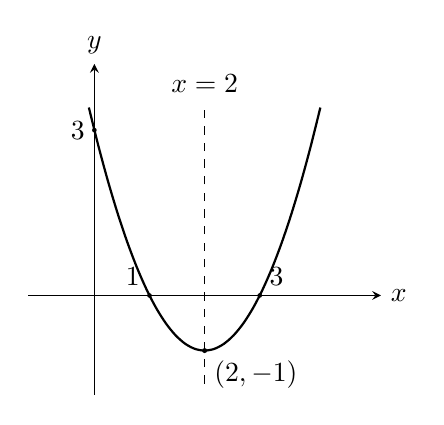
\begin{tikzpicture}[scale=0.7,>=stealth]
  \draw[->] (-1.2,0)--(5.2,0) node[right] {$x$};
  \draw[->] (0,-1.8)--(0,4.2) node[above] {$y$};
  \draw[thick,domain=-0.1:4.1,smooth,variable=\x]
    plot ({\x},{(\x-2)^2-1});
  \fill (2,-1) circle (1.3pt) node[below right] {$\left(2,-1\right)$};
  \fill (1,0) circle (1.2pt) node[above left] {$1$};
  \fill (3,0) circle (1.2pt) node[above right] {$3$};
  \fill (0,3) circle (1.2pt) node[left] {$3$};
  \draw[dashed] (2,-1.6)--(2,3.5) node[above] {$x=2$};
\end{tikzpicture}
\end{center}
\nopagebreak[4]
\gksubpart{（3）}

\Needspace{5\baselineskip}
联立抛物线与直线 $y=x-3$：

\nopagebreak[4]
\[
x^2-4x+3=x-3
\Longleftrightarrow x^2-5x+6=0
\Longleftrightarrow (x-2)(x-3)=0.
\]

当 $x=2$ 时 $y=-1$，当 $x=3$ 时 $y=0$，故交点为 $(2,-1)\text{、}(3,0)$。

\gkanswer{答案（1）：顶点为 $(2,-1)$，对称轴为 $x=2$。}

\gkanswer{答案（2）：见解析版。}

\gkanswer{答案（3）：交点为 $(1,-2)$、$(3,0)$。}

\end{answer}